\documentclass[]{article}

% Imported Packages
%------------------------------------------------------------------------------
\usepackage{amssymb}
\usepackage{amstext}
\usepackage{amsthm}
\usepackage{amsmath}
\usepackage{enumerate}
\usepackage{fancyhdr}
\usepackage[margin=1in]{geometry}
\usepackage{graphicx}
%\usepackage{extarrows}
%\usepackage{setspace}
\usepackage{color}
\usepackage{float}
\usepackage{tabularx}
%------------------------------------------------------------------------------

% Header and Footer
%------------------------------------------------------------------------------
\pagestyle{plain}  
\renewcommand\headrulewidth{0.4pt}                                      
\renewcommand\footrulewidth{0.4pt}                                    
%------------------------------------------------------------------------------

% Title Details
%------------------------------------------------------------------------------
\title{Deliverable \#2: What’s That Dish Software}
\author{SE 3A04: Software Design II -- Large System Design}
\date{}                           
%------------------------------------------------------------------------------

% Document
%------------------------------------------------------------------------------
\begin{document}

\maketitle	
\noindent{\bf Tutorial Number:} T03\\
{\bf Group Number:} G03 \\
{\bf Group Members:} 
\begin{itemize}
	\item Imran Chowdhury
	\item Michael Roberts
	\item Sathurshan Arulmohan
	\item Tanisha Tasnin
	\item Zifan Si
\end{itemize}

\section*{IMPORTANT NOTES}
\begin{itemize}
	%	\item You do \underline{NOT} need to provide a text explanation of each diagram; the diagram should speak for itself
	\item Please document any non-standard notations that you may have used
	\begin{itemize}
		\item \emph{Rule of Thumb}: if you feel there is any doubt surrounding the meaning of your notations, document them
	\end{itemize}
	\item Some diagrams may be difficult to fit into one page
	\begin{itemize}
		\item Ensure that the text is readable when printed, or when viewed at 100\% on a regular laptop-sized screen.
		\item If you need to break a diagram onto multiple pages, please adopt a system of doing so and thoroughly explain how it can be reconnected from one page to the next; if you are unsure about this, please ask about it
	\end{itemize}
	\item Please submit the latest version of Deliverable 1 with Deliverable 2
	\begin{itemize}
		\item Indicate any changes you made.
	\end{itemize}
	\item If you do \underline{NOT} have a Division of Labour sheet, your deliverable will \underline{NOT} be marked
\end{itemize}

\newpage
\section{Introduction}
\label{sec:introduction}
% Begin Section

\subsection{Purpose}
\label{sub:purpose}
% Begin SubSection
This document provides a highlevel overview of the system architecture for the What’s That Dish mobile application.
It provides insight into the classes required to build the application, along with the chosen architectural style for the system and its subsystems.
\\
\\
This document is intended for internal stakeholders of \textit{What’s That Dish}, which includes software architects, software developers, QA testers, and the project manager.
\\
\\
It is recommended that Deliverable 1 be reviewed in advance to gain a clear understanding of the application’s use cases, as well as its functional and non-functional requirements.
% End SubSection

\subsection{System Description}
\label{sub:system_description}
% Begin SubSection
\textit{What’s That Dish} is a mobile application designed for food identification, recipe management, and personalized recommendations. The system follows a modified Model-View-Controller (MVC) architecture, where user interactions are processed through controllers before being directed to specialized subsystems. This approach was chosen for its clear separation of concerns, improving maintainability and scalability while allowing each subsystem to operate independently with its own specialized architecture.
\\
\\
A variety of architectural styles, including Blackboard, Pipe-and-Filter, and Repository, can be seen across the subsystems. The application's core functionality, Dish Determination, utilizes the Blackboard architecture, involving the hypothesis-driven decision making of 3 independent expert modules for accurate food identification.
% End SubSection

\subsection{Overview}
\label{sub:overview}
% Begin SubSection
Section 2 presents the Analysis Class diagram for What's That Dish application.
Section 3 outlines the architectural design covering both the overall system architecture and its individual subsytems.
Section 4 provides Class Responsibility Collaboration cards for each class defined in the Analysis Class diagram.
% End SubSection

% End Section

\section{Analysis Class Diagram}
\label{sec:analysis_class_diagram}
% Begin Section
\begin{figure}[H]
	\centering
   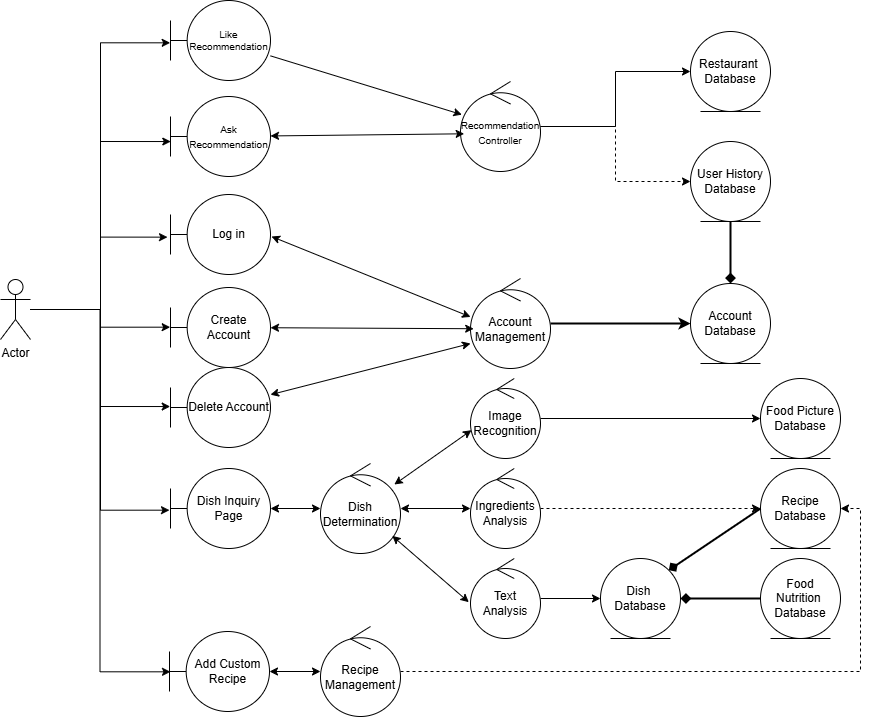
\includegraphics[width=\textwidth]{image/D2_2_analysis_class_diagram.png}
\end{figure}
% End Section


\section{Architectural Design}
\label{sec:architectural_design}
% Begin Section
This section should provide an overview of the overall architectural design of your application. Your overall architecture should show the division of the system into subsystems with high cohesion and low coupling.

\subsection{System Architecture}
\label{sub:system_architecture}
% Begin SubSection
\textit{What’s That Dish} follows a modified MVC (Model-View-Controller) approach, in which user interaction (View) first flows through a layer of Controllers that handle input and validation, then passes onto respective Model subsystems based on the user input. 
Each model subsystem follows independent and individual architectural styles. 
Dish Determination uses a Blackboard setup for its expert-based, iterative logic. 
Recipe Management applies a Pipe \& Filter workflow to sequentially process user‐submitted recipes. 
Recommendation and Account Management both rely on Repository principles, centralizing data for dynamic suggestions and secure credential handling. 
This layered organization preserves organization and clarity, allowing each subsystem to follow a specialized architecture suited to its unique requirements.
\\
\\
\\
What’s That Dish is defined by the following subsystems: 
\\
\\
\begin{tabularx}{1.0\textwidth} { 
  | >{\centering\arraybackslash}X 
  | >{\centering\arraybackslash}X 
  | >{\centering\arraybackslash}X | }
 \hline
 \textbf{Subsystem} & \textbf{Purpose} & \textbf{Architecture} \\
 \hline
 Dish Determination  & Identifies dishes using images, text, or ingredients  & Blackboard  \\
\hline
 Recipe Management  & Allows users to add and manage personal recipes  & Pipe-and-Filter  \\
\hline
 Recommendation System  & Suggests food and restaurant options based on user preferences  & Repository  \\
\hline
 Account Management  & Handles user authentication, account creation, and data storage  & Repository  \\
\hline

\end{tabularx}
\\
\\
\\
\textit{Please refer to section 3.2 for a more detailed classification of each subsystem.}
\\
\\
Dish Determination is characterized by complex decision-making based on 3 modules, Image Recognition, Text Description, and Ingredient-Based Experts, acting as independent and swappable knowledge sources, making Blackboard the ideal architecture style for this subsystem. 
The Dish Determination system actively evaluates and combines inputs from the modules and has internal controller embedded within it that is responsible for aggregating these inputs and managing confidence levels to determine the most accurate dish identification. 
This controller incorporates a Forum component, which is triggered when conflicting answers from expert modules arise.
It then proceeds to resolve the conflicting inputs from experts, ensuring that the final output is the most reliable identification based on computed confidence scores. 
The Forum here acts as a concluding mechanism by analyzing confidence levels in controller responses, a key property of the Blackboard model. 
This flexibility allows the system to aggregate expert inputs in real-time, ensuring a non-deterministic yet accurate output.  
To support this process, the Blackboard model’s asynchronous and parallel execution allows expert modules to efficiently handle incomplete or conflicting inputs without adhering to a rigid sequence of operations. 
It also offers scalability for future expansion, allowing new expert modules to be integrated easily without modifying the entire architecture.
\\
\\
Each innovative feature is built on top of the main functionality and follows its own architectural style.
\\
\\
Recipe Management implements the Pipe and Filter style. 
This architecture is well-suited for handling user-submitted recipes, as it allows data to flow through a sequence of independent processing stages (filters) connected by data streams (pipes). 
Each filter performs a specific function, such as validating inputs, analyzing ingredients, categorizing recipes, and storing data in the database, ensuring that recipes are properly formatted and classified. 
\\
\\
The Recommendation System adopts a Multi-Layered Architecture, allowing it to process user history, feedback, and external restaurant data separately from the storage layer. 
This separation is essential for automatically generating, updating, and refining personalized recommendations based on evolving user interactions.
\\
\\
Account Management uses the Repository architecture, where a centralized database stores user credentials and activity history. 
The database acts as a passive storage component, while the clients remain active, meaning that all processing and logic execution occur on the client side. 
This enables concurrent access and system-wide data sharing, providing real-time updates, and facilitating data integrity across different subsystems.
\\
\\
\begin{figure}[H]
    \centering
    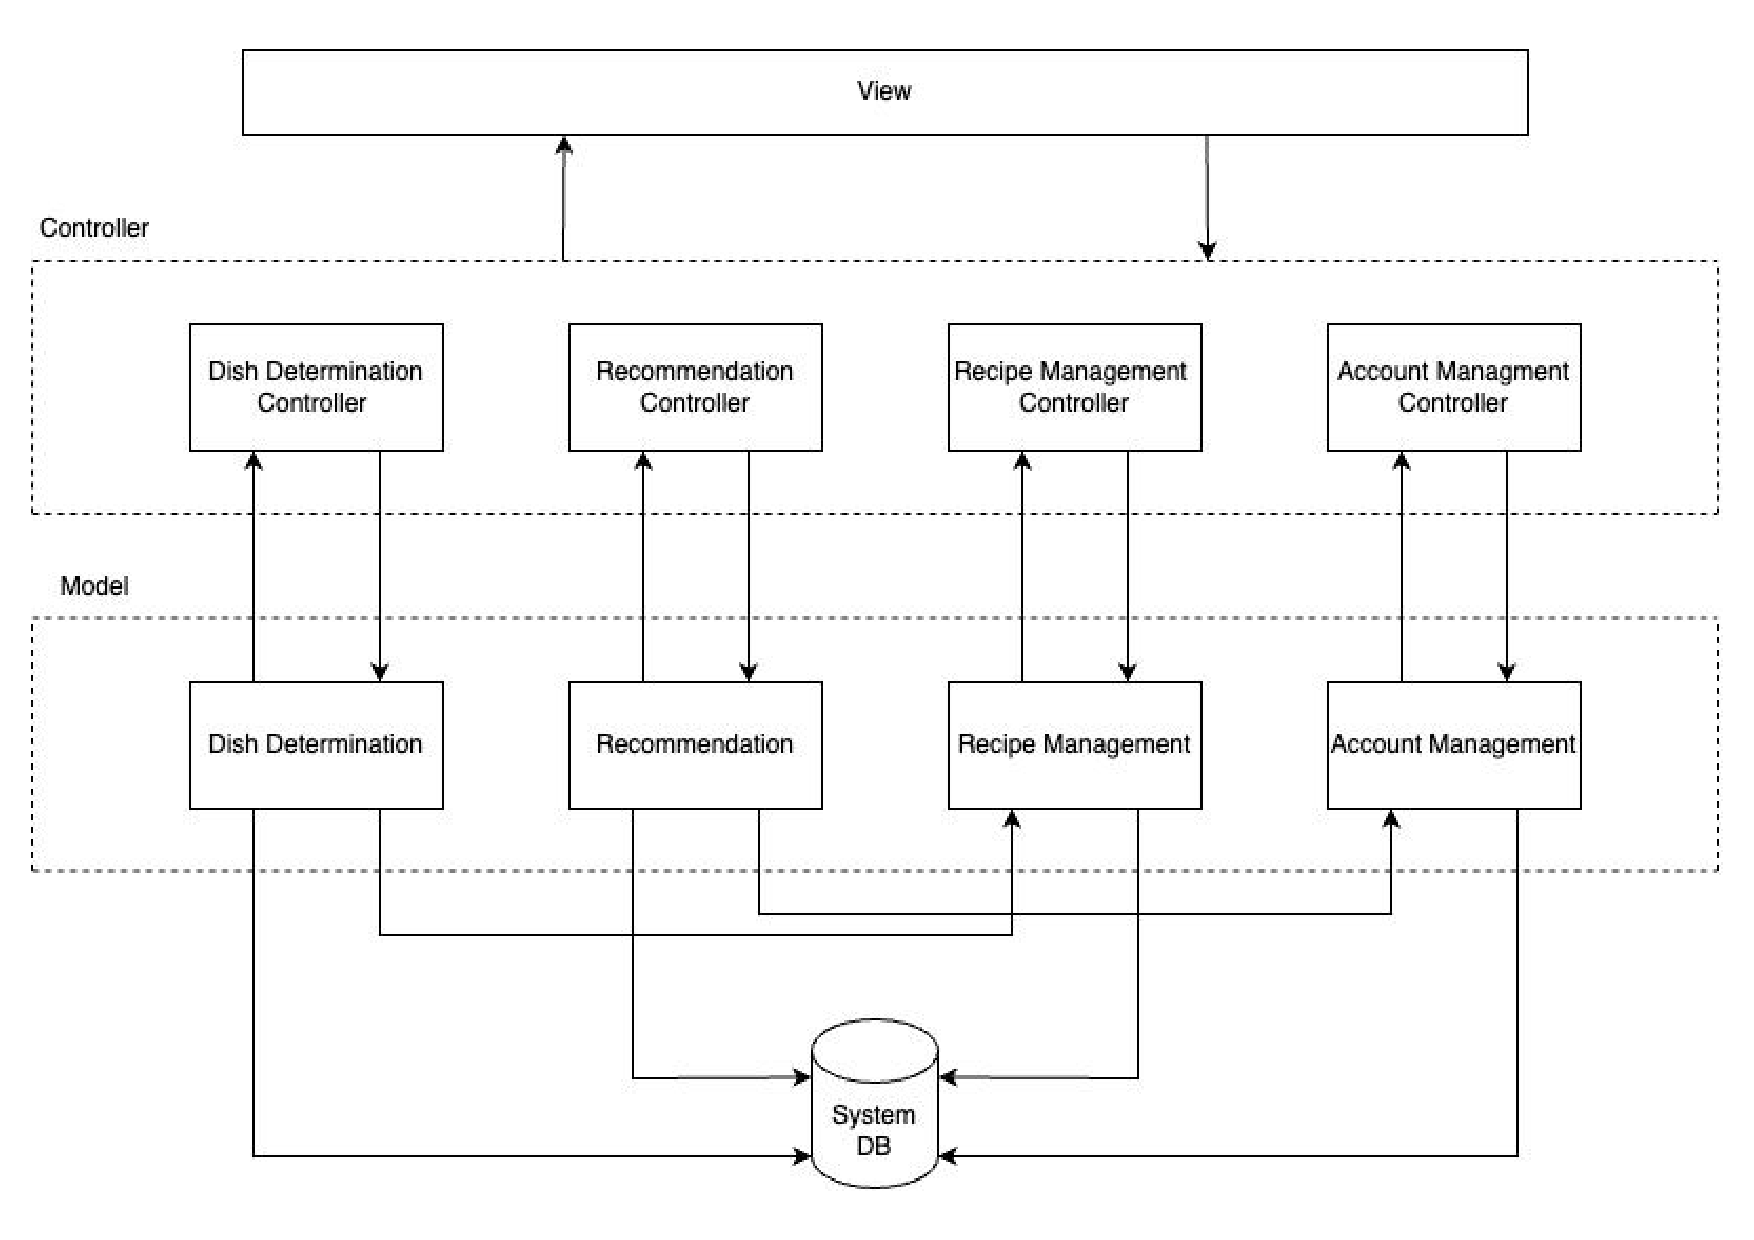
\includegraphics[width=\textwidth]{image/3.1_system_arch.pdf}
    \caption{\textbf{Figure 2. System Architecture}}
\end{figure}
\textit{The remainder of  3.1 explores other architectural styles that were strongly considered but ultimately found unsuitable due to certain limitations.}
\\
\\
An alternative architectural style considered for Dish Determination was the Pipe and Filter, where each expert module would function as a filter within the pipeline. 
However, Dish Determination requires modules to engage selectively based on the available input (e.g. bypassing Image Recognition when only an ingredient list is submitted), which conflicts with the rigid, linear data flow of Pipe and Filter. 
Another major drawback of Pipe and Filter is its lack of iterative refinement. 
Dish Determination involves conflict resolution, where different expert modules may generate contradictory results that require reevaluation. 
For instance, Text-Based Analysis may classify a dish differently than Image Recognition, requiring an additional layer of validation before presenting a final result. 
Pipe and Filter does not naturally support this kind of feedback loop, as data flows in a single direction, preventing experts from revising their outputs based on additional context.
This makes real-time accuracy adjustments and progressive refinement of food identifications difficult.
\\
\\
Batch Sequential was initially considered for Recipe Management, where user-submitted recipes would be processed in discrete batches rather than in a continuous flow. 
Under this approach, recipe submissions would be collected over time and processed periodically in bulk, undergoing validation, ingredient analysis, categorization, and storage as a group rather than individually. 
However, this method would introduce delays in recipe availability, reducing real-time user engagement. 
\\
\\
Model-View-Controller was contemplated for the Recommendation System due to its separation of concerns, which would allow the recommendation logic to operate independently from the UI for better maintainability.
However, MVC is best suited for applications with frequent user-driven interactions, whereas the Recommendation System relies on continuous data processing and real-time analysis rather than direct user input. 
Since the system must continually analyze user preferences, feedback, and external restaurant data to generate personalized suggestions, the Multi-Layered Repository approach is more suitable. 
This architecture supports efficient data flow, modular processing, and adaptability, ensuring consistent updates and refinements to recommendations as user data evolves.
% End SubSection

\subsection{Subsystems}
\label{sub:subsystems}
% Begin SubSection

The \textit{What’s That Dish} system is composed of multiple subsystems that work together to manage user accounts, provide dish recommendations, identify dishes, and manage databases. Each subsystem operates within a loosely coupled architecture to ensure modularity, maintainability, and scalability.

\subsubsection{Account Management Subsystem}
The Account Management subsystem is responsible for handling user authentication, account creation, deletion, and profile management. It provides functionalities such as logging in, extracting user data, and managing stored profiles. The system maintains user information within the Account Database.

\subsubsection{Recommendation Subsystem}
The Recommendation Controller subsystem provides dish recommendations based on user preferences, past interactions, and restaurant availability. It updates internal user recommendation history, tracks liked dishes, and communicates with restaurant databases to find suitable dining options.

\subsubsection{Dish Determination Subsystem}
The Dish Determination subsystem manages the process of dish identification based on user input. It collects dish-related data, processes it using various analytical techniques, and returns the final dish identification results to the Dish Inquiry page. It acts as a central hub, controlling the analysis of dish-related data.


\subsubsection{Image Recognition Subsystem}
The Image Recognition subsystem enables dish identification through image analysis. It uses a trained machine learning model to predict the dish name from an user uploaded picture. The Food Picture Database is utilized to improve the accuracy of dish predictions.


\subsubsection{Ingredients Analysis Subsystem}
The Ingredients Analysis subsystem predicts dish names based on ingredient lists provided by users. It cross-references user-inputted ingredients with recipes in the Recipe Database to identify potential dish matches.


\subsubsection{Text Analysis Subsystem}
The Text Analysis subsystem allows users to identify dishes based on textual descriptions. It performs semantic analysis on user-inputted text to predict the dish name accurately. The Dish Database stores structured dish information, which is used for comparisons.


\subsubsection{Recipe Management Subsystem}
The Recipe Management subsystem allows users to add and manage custom recipes. It ensures the proper organization and retrieval of user-submitted and system-generated recipes, storing all information in the Recipe Database.

% End SubSection

% End Section
	
\section{Class Responsibility Collaboration (CRC) Cards}
\label{sec:class_responsibility_collaboration_crc_cards}
% Begin Section

\begin{table}[H]
	\centering
	\begin{tabular}{|p{7cm}|p{7cm}|}
	\hline 
	 \multicolumn{2}{|l|}{\textbf{Class Name:} Create Account (Boundary)} \\
	\hline
	\textbf{Responsibility:} & \textbf{Collaborators:} \\
	\hline
	\raggedright
	\begin{itemize}
		\item Creates accounts
	\end{itemize}
	\vspace{1in} & 
	\begin{itemize}
		\item Account Management
	\end{itemize} \\
	\hline
	\end{tabular}
\end{table}

\begin{table}[H]
	\centering
	\begin{tabular}{|p{7cm}|p{7cm}|}
	\hline 
	 \multicolumn{2}{|l|}{\textbf{Class Name:} Delete account (Boundary)} \\
	\hline
	\textbf{Responsibility:} & \textbf{Collaborators:} \\
	\hline
	\raggedright
	\begin{itemize}
		\item Handles the event of a user deleting their account
	\end{itemize}
	\vspace{1in} & 
	\begin{itemize}
		\item Account Management
	\end{itemize} \\
	\hline
	\end{tabular}
\end{table}

\begin{table}[H]
	\centering
	\begin{tabular}{|p{7cm}|p{7cm}|}
	\hline 
	 \multicolumn{2}{|l|}{\textbf{Class Name:} Like Recommendation (Boundary)} \\
	\hline
	\textbf{Responsibility:} & \textbf{Collaborators:} \\
	\hline
	\raggedright
	\begin{itemize}
		\item Handles the "click" event of a user pressing the "Like" button
	\end{itemize}
	\vspace{1in} & 
	\begin{itemize}
		\item Recommendation Controller
	\end{itemize} \\
	\hline
	\end{tabular}
\end{table}

\begin{table}[H]
	\centering
	\begin{tabular}{|p{7cm}|p{7cm}|}
	\hline 
	 \multicolumn{2}{|l|}{\textbf{Class Name:} Ask Recommendation (Boundary)} \\
	\hline
	\textbf{Responsibility:} & \textbf{Collaborators:} \\
	\hline
	\raggedright
	\begin{itemize}
		\item Provides users recommendations based on user search history
	\end{itemize}
	\vspace{1in} & 
	\begin{itemize}
		\item Recommendation Controller
	\end{itemize} \\
	\hline
	\end{tabular}
\end{table}

\begin{table}[H]
	\centering
	\begin{tabular}{|p{7cm}|p{7cm}|}
	\hline 
	 \multicolumn{2}{|l|}{\textbf{Class Name:} Dish Inquiry Page (Boundary)} \\
	\hline
	\textbf{Responsibility:} & \textbf{Collaborators:} \\
	\hline
	\raggedright
	\begin{itemize}
		\item Handles the event of a user inputting dish information and the system outputting results to the user
	\end{itemize}
	\vspace{1in} & 
	\begin{itemize}
		\item Dish Determination
	\end{itemize} \\
	\hline
	\end{tabular}
\end{table}

\begin{table}[H]
	\centering
	\begin{tabular}{|p{7cm}|p{7cm}|}
	\hline 
	 \multicolumn{2}{|l|}{\textbf{Class Name:} Add Custom Recipe (Boundary)} \\
	\hline
	\textbf{Responsibility:} & \textbf{Collaborators:} \\
	\hline
	\raggedright
	\begin{itemize}
		\item Handles user request to add recipe
	\end{itemize}
	\vspace{1in} & 
	\begin{itemize}
		\item Recipe Management
	\end{itemize} \\
	\hline
	\end{tabular}
\end{table}

% Controller Classes

\begin{table}[H]
	\centering
	\begin{tabular}{|p{7cm}|p{7cm}|}
	\hline 
	 \multicolumn{2}{|l|}{\textbf{Class Name:} Recommendation Controller} \\
	\hline
	\textbf{Responsibility:} & \textbf{Collaborators:} \\
	\hline
	\raggedright
	\begin{itemize}
		\item Provides recommendation of dishes
		\item  Provides restarants serving recommended dish
		\item Updates internal user recommendation history
		\item Updates user liked dishes
	\end{itemize}
	\vspace{1in} & 
	\begin{itemize}
		\item Like Recommendation Boundary
		\item Ask Recommendation Boundary
		\item Restaurant Database
		\item User History Database
	\end{itemize} \\
	\hline
	\end{tabular}
\end{table}

\begin{table}[H]
	\centering
	\begin{tabular}{|p{7cm}|p{7cm}|}
	\hline 
	 \multicolumn{2}{|l|}{\textbf{Class Name:} Account Mangament} \\
	\hline
	\textbf{Responsibility:} & \textbf{Collaborators:} \\
	\hline
	\raggedright
	\begin{itemize}
		\item Knows log in
		\item  Provides restarants serving recommended dish
		\item Updates internal user recommendation history
		\item Updates user liked dishes
	\end{itemize}
	\vspace{1in} & 
	\begin{itemize}
		\item Like Recommendation Boundary
		\item Ask Recommendation Boundary
		\item Restaurant Database
		\item User History Database
	\end{itemize} \\
	\hline
	\end{tabular}
\end{table}

% Controllers

% Controller Classes
\begin{table}[H]
	\centering
	\begin{tabular}{|p{7cm}|p{7cm}|}
	\hline 
	 \multicolumn{2}{|l|}{\textbf{Class Name: Recommendation Controller}} \\
	\hline
	\textbf{Responsibility:} & \textbf{Collaborators:} \\
	\hline
	\raggedright
	\begin{itemize}
		\item Provides recommendation of dishes
		\item Provides restarants serving recommended dish
		\item Updates internal user recommendation history
		\item Updates user liked dishes
	\end{itemize}
	\vspace{1in} & 
	\begin{itemize}
		\item Like Recommendation Boundary
		\item Ask Recommendation Boundary
		\item Restaurant Database
		\item User History Database
	\end{itemize} \\
	\hline
	\end{tabular}
\end{table}

\begin{table}[H]
	\centering
	\begin{tabular}{|p{7cm}|p{7cm}|}
	\hline 
	 \multicolumn{2}{|l|}{\textbf{Class Name: Account Management (Controller)}} \\
	\hline
	\textbf{Responsibility:} & \textbf{Collaborators:} \\
	\hline
	\raggedright
	\begin{itemize}
		\item Manage accounts
		\item Handles log into user profile
		\item Extract user data
	\end{itemize}
	\vspace{1in} & 
	\begin{itemize}
		\item Account Database
	\end{itemize} \\
	\hline
	\end{tabular}
\end{table}

\begin{table}[H]
	\centering
	\begin{tabular}{|p{7cm}|p{7cm}|}
	\hline 
	 \multicolumn{2}{|l|}{\textbf{Class Name: Dish Determination (Controller)}} \\
	\hline
	\textbf{Responsibility:} & \textbf{Collaborators:} \\
	\hline
	\raggedright
	\begin{itemize}
		\item Manage the determination of a dish process
		\item Control the clients that determine the dish
		\item Accept dish data
		\item Provide dish information to Dish Inquiry Page
	\end{itemize}
	\vspace{1in} & 
	\begin{itemize}
		\item Dish Inquiry Page
		\item Image Recognition
		\item Ingredients Analysis
		\item Text Analysis
	\end{itemize} \\
	\hline
	\end{tabular}
\end{table}

\begin{table}[H]
	\centering
	\begin{tabular}{|p{7cm}|p{7cm}|}
	\hline 
	 \multicolumn{2}{|l|}{\textbf{Class Name: Image Recognition (Controller)}} \\
	\hline
	\textbf{Responsibility:} & \textbf{Collaborators:} \\
	\hline
	\raggedright
	\begin{itemize}
		\item Predict dish from picture
	\end{itemize}
	\vspace{1in} & 
	\begin{itemize}
		\item Dish Determination
		\item Food Picture Database
	\end{itemize} \\
	\hline
	\end{tabular}
\end{table}

\begin{table}[H]
	\centering
	\begin{tabular}{|p{7cm}|p{7cm}|}
	\hline 
	 \multicolumn{2}{|l|}{\textbf{Class Name: Ingredients Analysis (Controller)}} \\
	\hline
	\textbf{Responsibility:} & \textbf{Collaborators:} \\
	\hline
	\raggedright
	\begin{itemize}
		\item Predict dish from ingredients list.
	\end{itemize}
	\vspace{1in} & 
	\begin{itemize}
		\item Dish Determination
		\item Recipe Database
	\end{itemize} \\
	\hline
	\end{tabular}
\end{table}

\begin{table}[H]
	\centering
	\begin{tabular}{|p{7cm}|p{7cm}|}
	\hline 
	 \multicolumn{2}{|l|}{\textbf{Class Name: Text Analysis (Controller)}} \\
	\hline
	\textbf{Responsibility:} & \textbf{Collaborators:} \\
	\hline
	\raggedright
	\begin{itemize}
		\item Predict dish from text semantic analysis
	\end{itemize}
	\vspace{1in} & 
	\begin{itemize}
		\item Dish Determination
		\item Dish Database
	\end{itemize} \\
	\hline
	\end{tabular}
\end{table}

\begin{table}[H]
	\centering
	\begin{tabular}{|p{7cm}|p{7cm}|}
	\hline 
	 \multicolumn{2}{|l|}{\textbf{Class Name: Recipe Management (Controller)}} \\
	\hline
	\textbf{Responsibility:} & \textbf{Collaborators:} \\
	\hline
	\raggedright
	\begin{itemize}
		\item Manage the Recipe Database.
		\item Accept new recipes
	\end{itemize}
	\vspace{1in} & 
	\begin{itemize}
		\item Add Custom Recipe Boundary
		\item Recipe Database
	\end{itemize} \\
	\hline
	\end{tabular}
\end{table}

% Entities

\begin{table}[H]
	\centering
	\begin{tabular}{|p{7cm}|p{7cm}|}
	\hline 
	 \multicolumn{2}{|l|}{\textbf{Class Name:} Restaurant Database (Entity) }\\
	\hline
	\textbf{Responsibility:} & \textbf{Collaborators:} \\
	\hline
	\raggedright
	\begin{itemize}
		\item Knows data about restaurants (e.g. name, address, type)
	\end{itemize}
	\vspace{1in} & 
	\begin{itemize}
		\item Recommendation Controller
	\end{itemize} \\
	\hline
	\end{tabular}
\end{table}

\begin{table}[H]
	\centering
	\begin{tabular}{|p{7cm}|p{7cm}|}
	\hline 
	 \multicolumn{2}{|l|}{\textbf{Class Name:} Account Database (Entity) }\\
	\hline
	\textbf{Responsibility:} & \textbf{Collaborators:} \\
	\hline
	\raggedright
	\begin{itemize}
		\item Knows data about accounts (e.g. username, password, email)
		\item Stores subset data about user history.
	\end{itemize}
	\vspace{1in} & 
	\begin{itemize}
		\item Account Management
	\end{itemize} \\
	\hline
	\end{tabular}
\end{table}

\begin{table}[H]
	\centering
	\begin{tabular}{|p{7cm}|p{7cm}|}
	\hline 
	 \multicolumn{2}{|l|}{\textbf{Class Name:} User History Database (Entity) }\\
	\hline
	\textbf{Responsibility:} & \textbf{Collaborators:} \\
	\hline
	\raggedright
	\begin{itemize}
		\item Knows history about accounts (e.g. like history, browsing history)
	\end{itemize}
	\vspace{1in} & 
	\begin{itemize}
		\item Recommendation Controller
		\item Account Database
	\end{itemize} \\
	\hline
	\end{tabular}
\end{table}

\begin{table}[H]
	\centering
	\begin{tabular}{|p{7cm}|p{7cm}|}
	\hline 
	 \multicolumn{2}{|l|}{\textbf{Class Name:} Food Picture Database (Entity) }\\
	\hline
	\textbf{Responsibility:} & \textbf{Collaborators:} \\
	\hline
	\raggedright
	\begin{itemize}
		\item Knows labels to stored pictures of foods 
	\end{itemize}
	\vspace{1in} & 
	\begin{itemize}
		\item Image Analysis
	\end{itemize} \\
	\hline
	\end{tabular}
\end{table}

\begin{table}[H]
	\centering
	\begin{tabular}{|p{7cm}|p{7cm}|}
	\hline 
	 \multicolumn{2}{|l|}{\textbf{Class Name:} Dish Database (Entity) }\\
	\hline
	\textbf{Responsibility:} & \textbf{Collaborators:} \\
	\hline
	\raggedright
	\begin{itemize}
		\item Contains Dish information such as name, food fasct, nutrients, recipes, and origin.
	\end{itemize}
	\vspace{1in} & 
	\begin{itemize}
		\item Text Analysis
		\item Recipe Database
		\item Food Nutrition Database
	\end{itemize} \\
	\hline
	\end{tabular}
\end{table}

\begin{table}[H]
	\centering
	\begin{tabular}{|p{7cm}|p{7cm}|}
	\hline 
	 \multicolumn{2}{|l|}{\textbf{Class Name:} Recipe Database (Entity) }\\
	\hline
	\textbf{Responsibility:} & \textbf{Collaborators:} \\
	\hline
	\raggedright
	\begin{itemize}
		\item Knows recipes for dishes
	\end{itemize}
	\vspace{1in} & 
	\begin{itemize}
		\item Dish Database
		\item Ingredients Analysis
		\item Recipe Management
	\end{itemize} \\
	\hline
	\end{tabular}
\end{table}

\begin{table}[H]
	\centering
	\begin{tabular}{|p{7cm}|p{7cm}|}
	\hline 
	 \multicolumn{2}{|l|}{\textbf{Class Name:} Food Nutrition Database (Entity) }\\
	\hline
	\textbf{Responsibility:} & \textbf{Collaborators:} \\
	\hline
	\raggedright
	\begin{itemize}
		\item Knows nutrition facts for dishes
	\end{itemize}
	\vspace{1in} & 
	\begin{itemize}
		\item Dish Database
	\end{itemize} \\
	\hline
	\end{tabular}
\end{table}



% End Section

\appendix
\section{Division of Labour}
\label{sec:division_of_labour}
\textbf{Imran Chowdhury:}
\begin{enumerate}
	\item Brainstorming and drawing the strutural architecture diagram.
	\item Wrote and editted section 3.1.
	\item Ensured consistency in the document.
\end{enumerate}

\textbf{Signature:} Imran Chowdhury \\

\textbf{Michael Roberts:}
\begin{enumerate}
	\item TODO
\end{enumerate}

\begin{figure}[H]
 	\centering
    
\includegraphics[width=\textwidth]{image/A_Michael_Roberts_Signature.png}
\end{figure}

\textbf{Sathurshan Arulmohan:}
\begin{enumerate}
	\item Brainstorming and drawing the Analysis Class Diagram.
	\item Wrote section 1.1 and 1.3.
	\item Wrote CRC for controller classes
	\item Provided feedback for written portion of section 3.
\end{enumerate}

\textbf{Signature:} SATHURSHAN ARULMOHAN \\

\textbf{Tanisha Tasnin:}
\begin{enumerate}
	\item Wrote section 3.1 
	\item Provided feedback for Analysis Class Diagram
	\item Wrote section 1.2
\end{enumerate}

\textbf{Signature:} TANISHA TASNIN \\

\textbf{Zifan Si:}
\begin{enumerate}
	\item Wrote section 3.2.
\end{enumerate}

\textbf{Signature:} ZIFAN SI  \\


\end{document}
%------------------------------------------------------------------------------
